\usetikzlibrary{shapes.geometric}

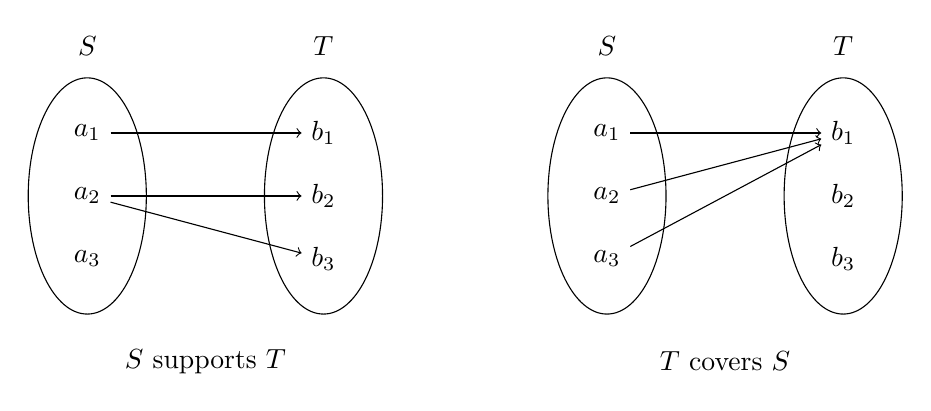
\begin{tikzpicture}


    \node[ellipse,
    draw = black,
    minimum width = 1.5cm, 
    minimum height = 3cm] (e) at (-4.8,0) {};

    \node[ellipse,
    draw = black,
    minimum width = 1.5cm, 
    minimum height = 3cm] (e) at (-1.8,0) {};

    \node[ellipse,
    draw = black,
    minimum width = 1.5cm, 
    minimum height = 3cm] (e) at (1.8,0) {};

    \node[ellipse,
    draw = black,
    minimum width = 1.5cm, 
    minimum height = 3cm] (e) at (4.8,0) {};


    \node[] (a1) at (-4.8,.8) {$a_1$};
    \node[] (a2) at (-4.8,0) {$a_2$};
    \node[] (a3) at (-4.8,-.8) {$a_3$};

    \node[] (a1') at (-1.8,.8) {$b_1$};
    \node[] (a2') at (-1.8,0) {$b_2$};
    \node[] (a3') at (-1.8,-.8) {$b_3$};

    \node[] (b1) at (4.8,.8) {$b_1$};
    \node[] (b2) at (4.8,0) {$b_2$};
    \node[] (b3) at (4.8,-.8) {$b_3$};

    \node[] (b1') at (1.8,.8) {$a_1$};
    \node[] (b2') at (1.8,0) {$a_2$};
    \node[] (b3') at (1.8,-.8) {$a_3$};

    \node[] (label) at (-3.3, -2.1) {$S$ supports $T$};
    \node[] (label) at (3.3, -2.1) {$T$ covers $S$};

    \node[] (label) at (-4.8, 1.9) {$S$};
    \node[] (label) at (-1.8, 1.9) {$T$};

    \node[] (label) at (1.8, 1.9) {$S$};
    \node[] (label) at (4.8, 1.9) {$T$};


      \draw[->] (a1) to (a1');
      \draw[->] (a2) to (a2');
      \draw[->] (a2) to (a3');

      \draw[->] (b1') to (b1);
      \draw[->] (b2') to (b1);
      \draw[->] (b3') to (b1);
  \end{tikzpicture}